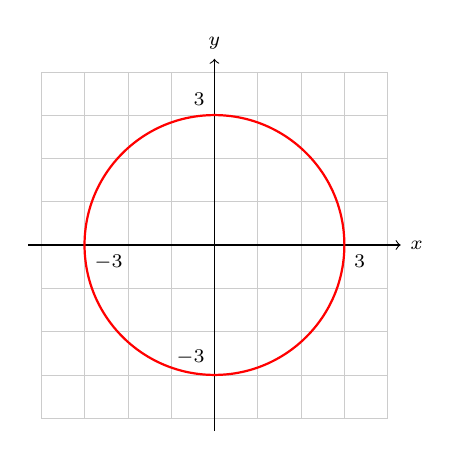
\begin{tikzpicture}[scale=0.55, every node/.style={font=\scriptsize}]
  \draw[gray!40, very thin] (-4,-4) grid (4,4);
  \draw[->] (-4.3,0) -- (4.3,0) node[right] {$x$};
  \draw[->] (0,-4.3) -- (0,4.3) node[above] {$y$};
  \foreach \x in {-3,3} \node[below right] at (\x,0) {$\x$};
  \foreach \y in {-3,3} \node[above left] at (0,\y) {$\y$};
  \draw[red, thick] (0,0) circle (3);
\end{tikzpicture}
